\NumberThisInToc
\chapter*{Conclusion}\label{chap:Conclu}

Dans ce manuscrit, nous avons présenté les différents travaux qui s'inscrivent directement dans le cadre d'une expérience ayant pour but la réalisation d'un \lat continu et intense.
Les différents axes de recherche qui ont été présentés ont donné lieu à la rédaction de 8 articles~\cite{LWR05,LRW06,RWC06,RLC06,CKR08,RLW07,CJK08,ReG08}, dont les références et résumés sont réunis dans l'annexe~\nref{annexe:Articles}.

%La première partie traite de la formation et de l'évaporation un \jatgm.

\newcommand{\figgg}[1]%
{#1}
\def\sssize{5.75cm}

\vspace{1ex}

\figgg{\inlinefigr{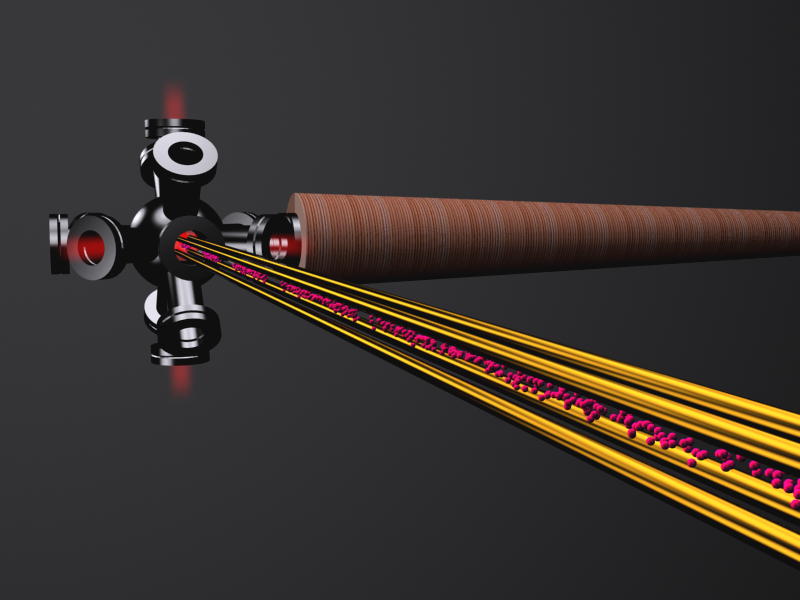
\includegraphics[width=\sssize]{P1/ChapitreJetAtomique}}}
Nous avons commencé dans le chapitre \ref{chap:JetAtomique} par décrire le \setup qui nous a permis de mettre en \oe uvre le \rpef d'un \jatuf \mg~\cite{LWR05}. Le gain d'un facteur $10$ sur la \ddedp semble faible face aux sept ordres de grandeur qui nous séparent encore de la \condbe. Le paramètre physique qui nous limite en définitive est le nombre moyen $\Ncol\approx20$ de collisions subies par un atome au cours de sa propagation dans le guide. 

Si nous pouvions disposer d'un nombre dix fois plus élevé de collisions, le \rdq serait probablement accessible. 
Nous avons donc conclu à la nécessité de développer de nouveaux outils visant à améliorer les conditions d'évaporation dans le \gm.

\vspace{1ex}
\vspace{1ex}

\figgg{\inlinefigr{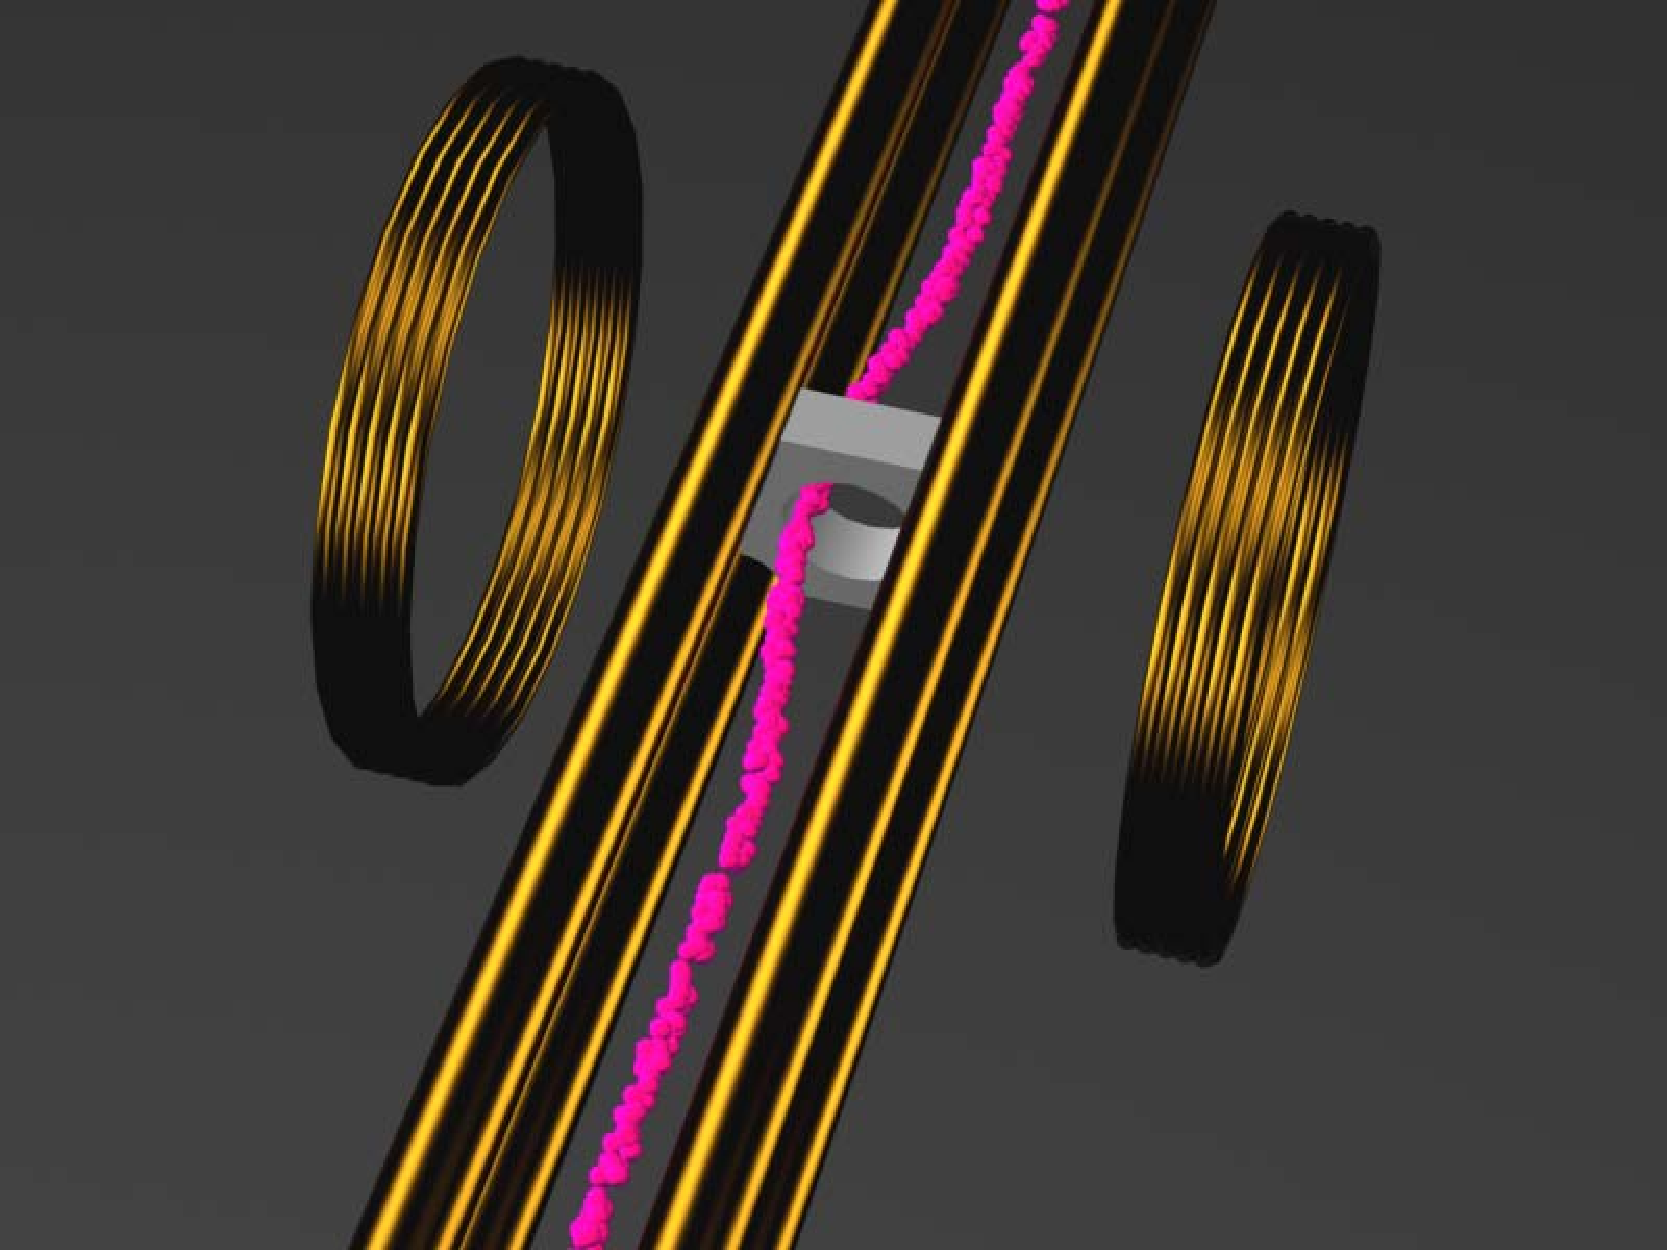
\includegraphics[width=\sssize]{P1/ChapitreCeramique}}}
Dans le chapitre \ref{chap:Ceramique} nous avons présenté une technique permettant de mener à bien l'\evap d'un \jatmg. Pour cela nous dévions localement la trajectoire du jet vers l'une des \pdecs présente dans notre \gm. 
Le contrôle de la déviation est assuré par la superposition local d'un \chm transverse à l'axe du guide~\cite{RLC06}. 

Ce processus d'évaporation peut, dans certaines conditions, être aisément rendu bidimensionnel et présente plusieurs avantages majeurs en comparaison de l'évaporation par \firf:
\begin{itemizel}
	\item l'efficacité de l'élimination des atomes répondant au critère de filtrage est de $100\%$,
	\item l'action de \fisp est beaucoup plus locale puisqu'elle se produit au contact de la surface, de quelques millimètres de long dans notre cas.
\end{itemizel}

\vspace{1ex}
\vspace{1ex}

\figgg{\inlinefigr{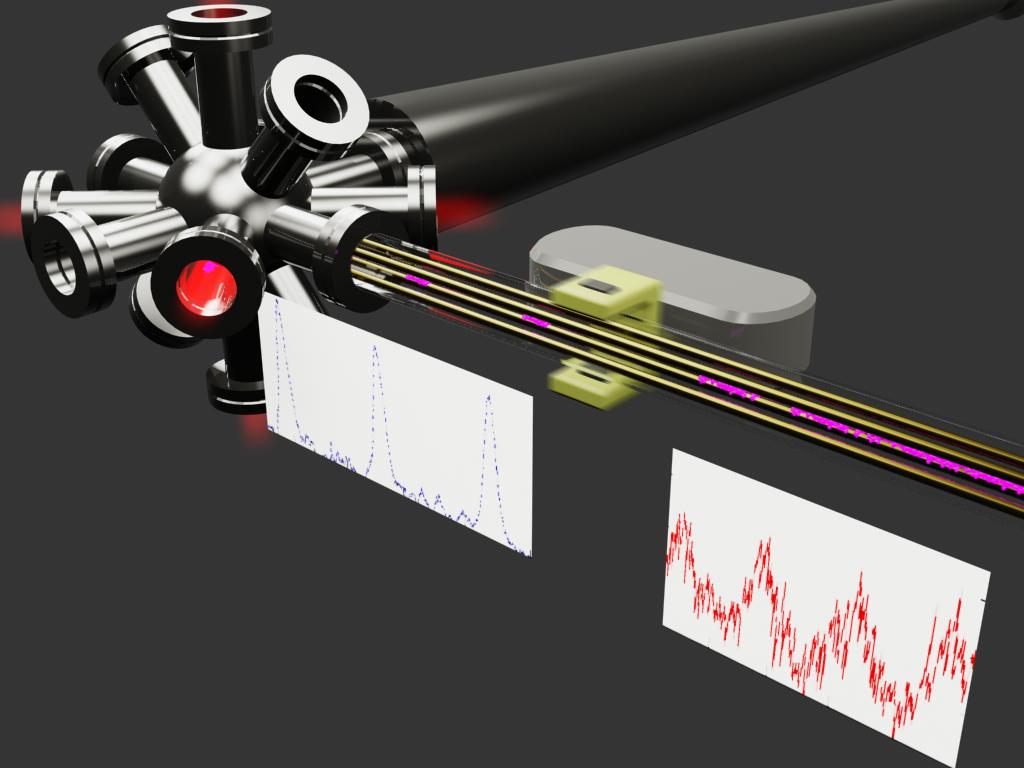
\includegraphics[width=\sssize]{P2/ChapitreMiroir}}}
Dans le chapitre \ref{chap:MiroirMobile},
nous avons décrit la mise en \oe uvre d'une technique de ralentissement des \pats par réflexion sur un \mimamo~\cite{RWC06}. 
%Nous avons démontré le ralentissement de \pat individuels, ainsi que d'une succession de \ps qui, se recouvrant par la suite, forment un \jat très lent. 

Nous avons souligné les paramètres à considérer afin de pouvoir, dans le futur,  concevoir une nouvelle expérience qui serait optimisée pour tirer pleinement partie des qualités de cette technique. Nous avons par ailleurs constaté que :
\begin{itemize}
	\item le ralentissement par réflexion n'augmente pas la\\ \dispvitlong des \ps,\\ contrairement à l'utilisation d'une \secpent,
	\item la \ddedpup du jet ainsi formé peut être supérieure à celle obtenue en l'absence de ralentissement, ou même à celle obtenue par l'utilisation d'une \secpent.
\end{itemize}
\picskip{0}
\noindent
Ce dernier point est remarquable et nous a amené à considérer l'action du \mimo sur les \ps comme celle d'un \termetech{démon de Maxwell}~\cite{ReG08}.

\vspace{1ex}
\vspace{1ex}

\figgg{\inlinefigr{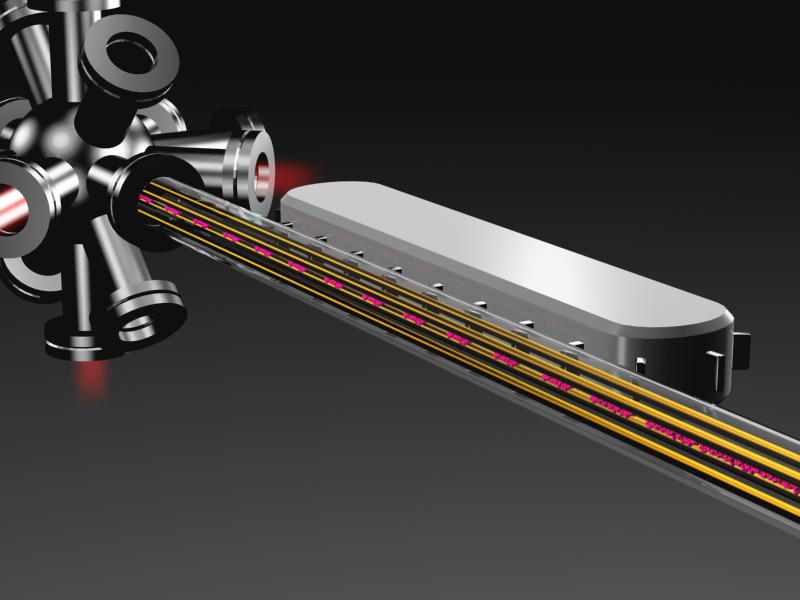
\includegraphics[width=\sssize]{P2/ChapitreConvoyeur}}}
Nous avons présenté dans le chapitre \ref{chap:Convoyeur}, la mise en \oe uvre d'un \tpIP mobiles. 
%Les paquets d'atomes injectés dans le guide y sont re-capturés dans un référentiel en mouvement. 
Nous avons observé expérimentalement le fait que la capture dans le \tp en mouvement permet de :
\begin{itemize}
	\item limiter la dilution longitudinale afin de maintenir\\ un \tcolel élevé,
	\item recréer des conditions de piégeage tridimensionnel, 
\end{itemize} 
et cela afin de bénéficier d'une évaporation plus efficace. De plus, nous pouvons envisager de ralentir les paquets lors de leur capture de manière à disposer, par suite, d'un \jat lent sur la dernière partie du guide.

Nous avons de plus mis en \oe uvre le \rpef sur $5$ paquets simultanément et avec une alimentation périodique du \tp~\cite{LRW06}. 
Ces expériences nous ont en outre permis de définir les paramètres critiques qui permettront sans doute la mise au point d'un futur \setup entièrement optimisé pour l'usage de cette technique. 

\vspace{1ex}
\vspace{1ex}

\figgg{\inlinefigr{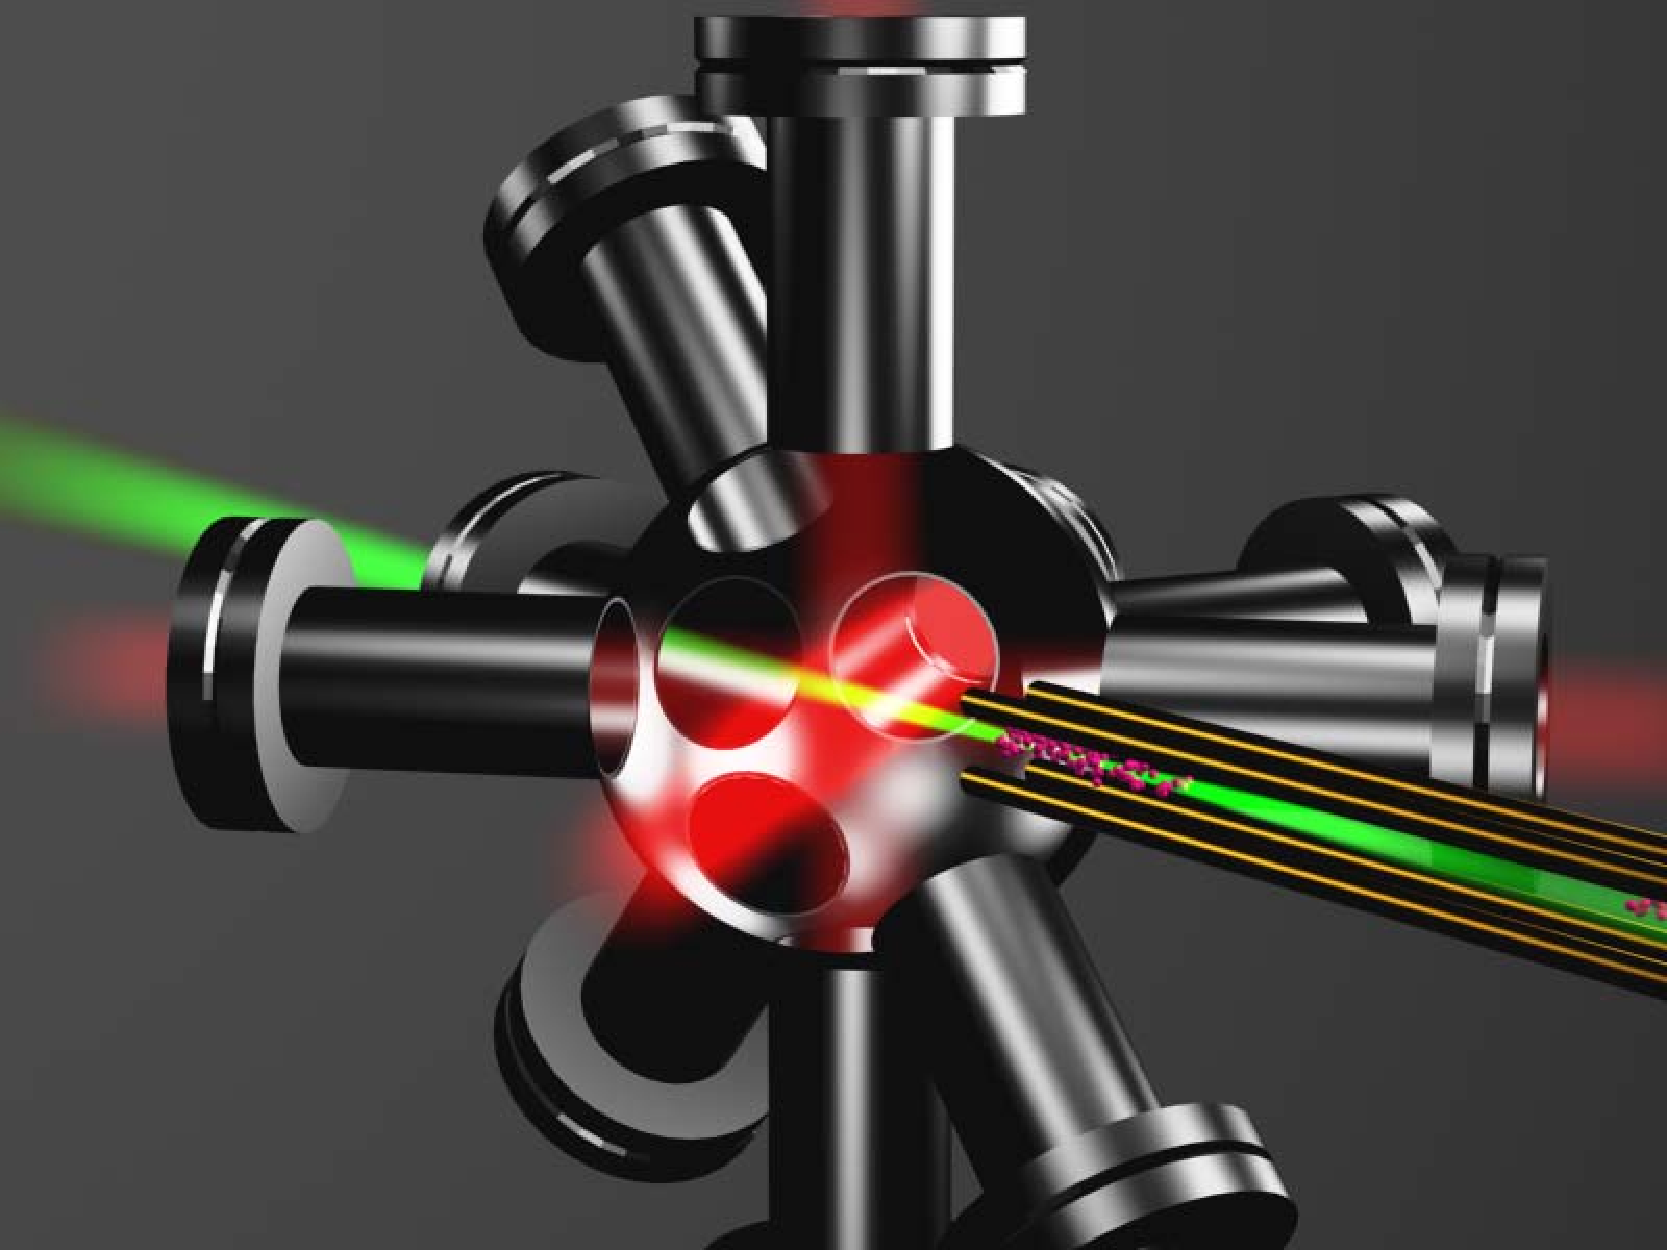
\includegraphics[width=\sssize]{P3/ChapitreMonster3ds286}}}
Nous avons montré dans le chapitre \ref{chap:PiegeDipolaire} qu'un \pd en faisceau unique semble être un outil adapté en ce qui concerne la \termetech{production}, puis à la \termetech{mise en mouvement} de \patufs et denses. 
Nous avons vu que, par un choix judicieux du \pacc et de la durée de la mise en mouvement, il est possible de déplacer un \nat rapidement et de manière \termetech{optimale}, \cad sans affecter ses caractéristiques après le mouvement~\cite{CKR08}.


\vspace{1ex}
\vspace{1ex}

\figgg{\inlinefigr{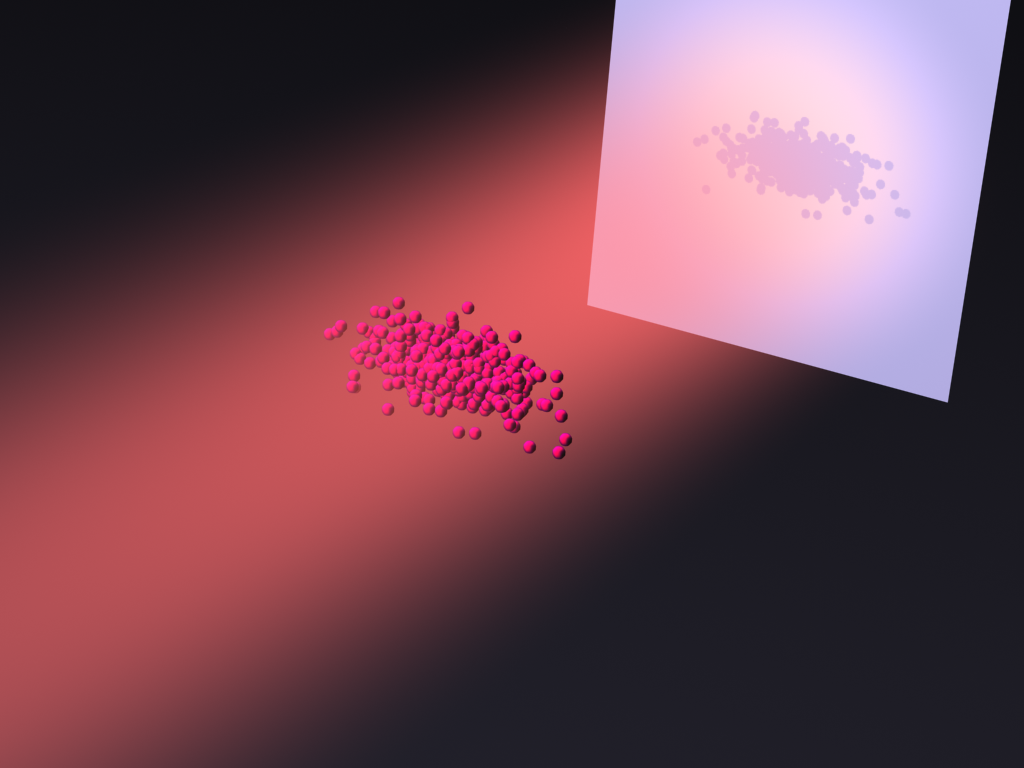
\includegraphics[width=\sssize]{P3/ChapitreImagerie}}}
Enfin, nous avons décrit, dans le 
chapitre \ref{chap:Imagerie}, un nouveau protocole d'imagerie. En effet, les deux techniques prédominantes pour faire l'image d'ensembles atomiques dilués, à savoir l'\termetech{imagerie par absorption à faible intensité} et l'\termetech{imagerie par fluorescence}, s'avèrent peu fiables lorsqu'il s'agit de traiter des \ns dont la \pro excède \val{4} ou \val{5}.
Notre protocole permet de résoudre les structures de \nats denses, et donne accès à des mesures quantitatives et précises~\cite{RLW07}. 
Le système optique nécessaire pour pouvoir l'appliquer est tout à fait standard.



\vspace{1ex}
\vspace{1ex}
\vspace{1ex}


Les résultats qui ont été présentés dans ce manuscrit sont encourageants quant à la perspective de concevoir un nouveau \setup qui pourrait combiner les techniques que nous avons développées. Celui-ci pourrait permettre de produire un \jat \uf et de mettre en \oe uvre le \rpef jusqu'à atteindre le \rdq. 

Soulignons par ailleurs le fait que les divers outils et méthodes développés lors de ces recherches s'avèrent avoir une portée plus générale et présentent un intérêt potentiel pour beaucoup d'expériences d'atomes froids. 






